\chapter{\babDua}
\section{Membuat penilaian diri}
Untuk membuat proyek penilaian diri pertama kali, klik dialog \texttt{List surveys} seperti \figurename~\ref{fig:masukPertama} atau melalui menu seperti \figurename~\ref{fig:createSurvey}.
\begin{figure}
  \begin{center}
    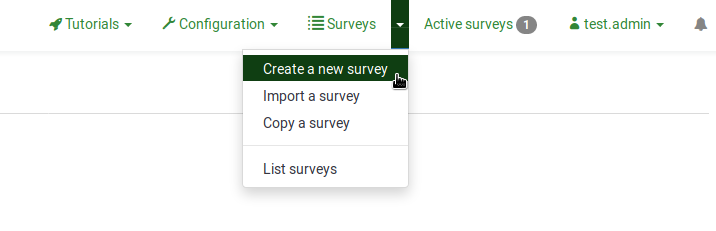
\includegraphics[scale=.45]{pics/createSurvey.png}
    \caption{Menu untuk membuat penilaian diri}
    \label{fig:createSurvey}
  \end{center}
\end{figure}

Selanjutnya, pengelola akan mendapati dialog seperti pada \figurename~\ref{fig:proyekSurvey}.
\begin{figure}
  \begin{center}
    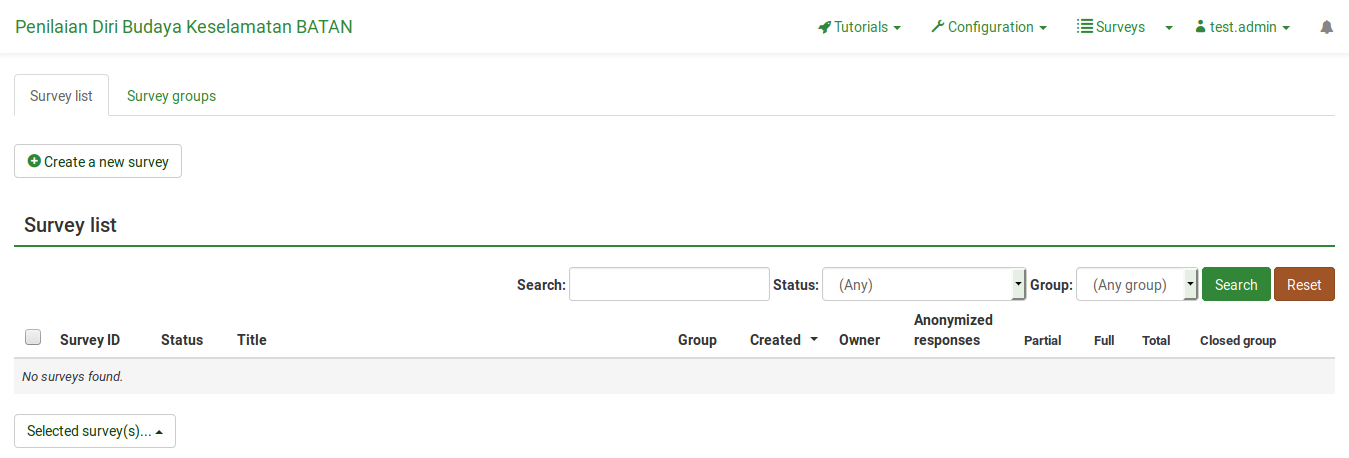
\includegraphics[scale=.35]{pics/proyekSurvey.png}
    \caption{Dialog yang menampilkan daftar penilaian diri}
    \label{fig:proyekSurvey}
  \end{center}
\end{figure}

\section{Membuat penilaian diri dari awal}
Yang dimaksud dengan membuat penilaian diri dari awal adalah membuatnya tidak berdasarkan \textit{template} penilaian diri yang pernah dibuat sebelumnya. Untuk melakukannya, pengelola dapat melakukan klik di menu \texttt{Create a new survey} seperti ditunjukkan pada \figurename~\ref{fig:proyekSurvey}. Setelahnya, pengelola akan mendapati dialog seperti \figurename~\ref{fig:proyekSurvey1}.

\begin{figure}
  \begin{center}
    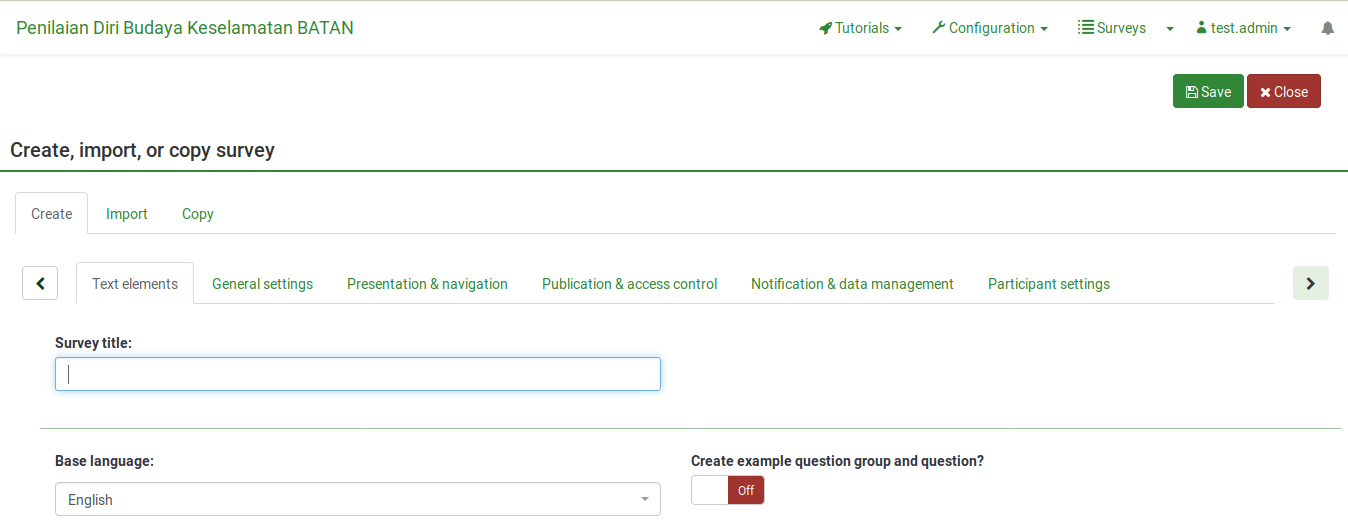
\includegraphics[scale=.35]{pics/proyekSurvey1.png}
    \caption{Dialog untuk membuat penilaian diri}
    \label{fig:proyekSurvey1}
  \end{center}
\end{figure}

Di \figurename~\ref{fig:proyekSurvey1}, terlihat tiga buah tab dengan judul \texttt{Create}, \texttt{Import} dan \texttt{Copy}. Dua tab terakhir digunakan ketika kita akan membuat penilaian diri berdasarkan \textit{template} penilaian diri yang pernah dibuat. Pengelola dapat memasukkan judul penilaian diri pada dialog seperti \figurename~\ref{fig:proyekSurvey1} kemudian menyimpannya dengan melakuan klik di tombol \texttt{Save}. Penilaian diri yang baru disimpan akan muncul dalam daftar penilaian diri seperti ditunjukkan \figurename~\ref{fig:daftarSurvey}.

\begin{figure}
  \begin{center}
    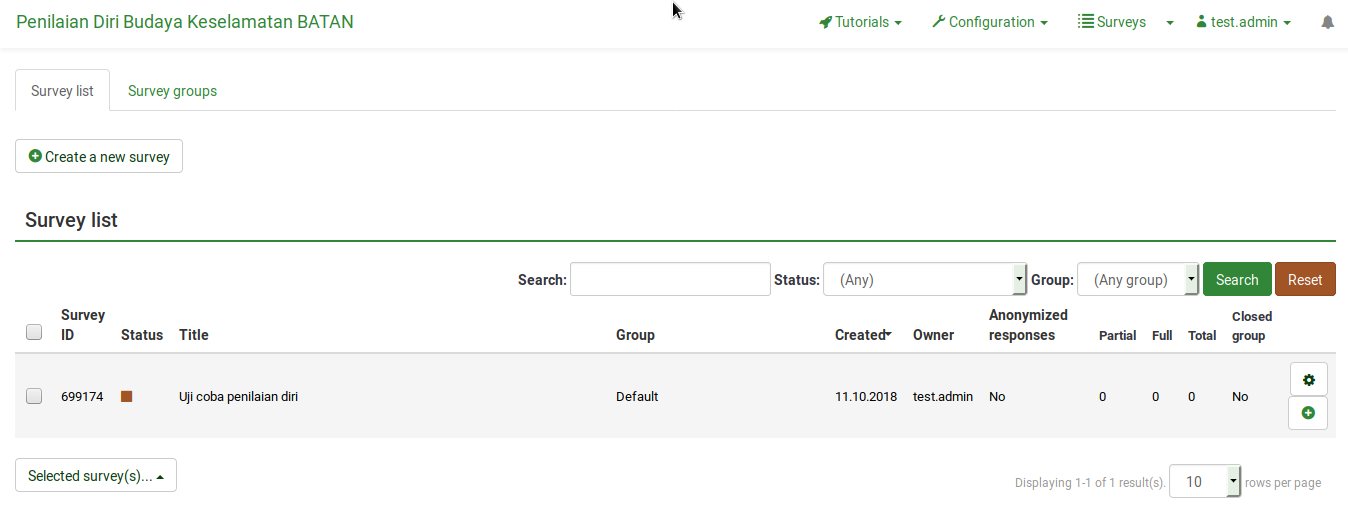
\includegraphics[scale=.35]{pics/daftarSurvey.png}
    \caption{Penilaian diri yang dibuat telah terdaftar}
    \label{fig:daftarSurvey}
  \end{center}
\end{figure}

Untuk memodifikasi penilaian diri lebih lanjut, silakan melakukan klik di baris penilaian diri yang diinginkan. Selanjutnyam pengelola akan menjumpai dialog seperti \figurename~\ref{fig:modifSurvey}. Modifikasi terkait pertanyaan yang akan diajukan dalam penilaian diri dilakukan melalui tab \texttt{Structure} (dengan lingkaran hitam). Sedangkan modifikasi lainnya dilakukan melalui tab \texttt{Settings}.

\begin{figure}
  \begin{center}
    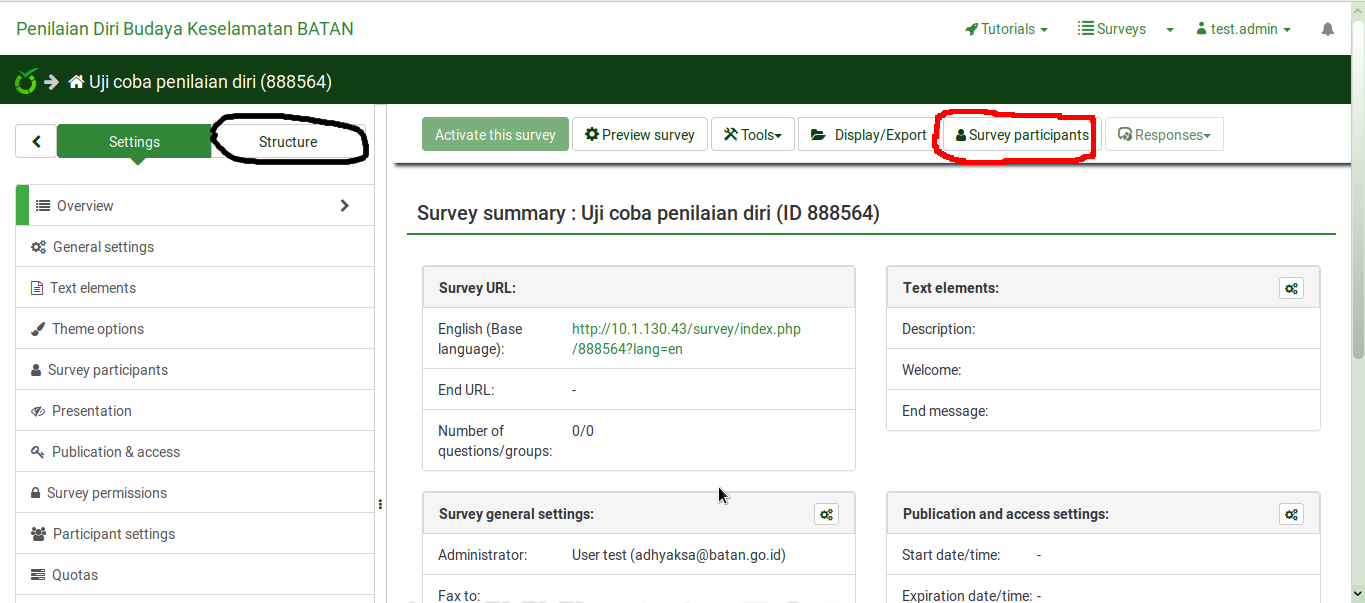
\includegraphics[scale=.4]{pics/proyekSurvey2.png}
    \caption{Memodifikasi penilaian diri}
    \label{fig:modifSurvey}
  \end{center}
\end{figure}

Jika klik diberikan pada menu \texttt{Structure} pada \figurename~\ref{fig:modifSurvey}, dialog seperti pada \figurename~\ref{fig:addGroupStructure} akan muncul. Informasi yang harus disediakan adalah judul dari \texttt{question group}. Pengelola dapat menyimpannya untuk kemudian menambahkan pertanyaan penilaian diri di \texttt{question group} yang baru saja dibuat atau melanjutkan penambahan \texttt{question group} berikutnya. Tombol untuk menyimpannya ada di pojok kanan atas dari \figurename~\ref{fig:addGroupStructure}.

\begin{figure}
  \begin{center}
    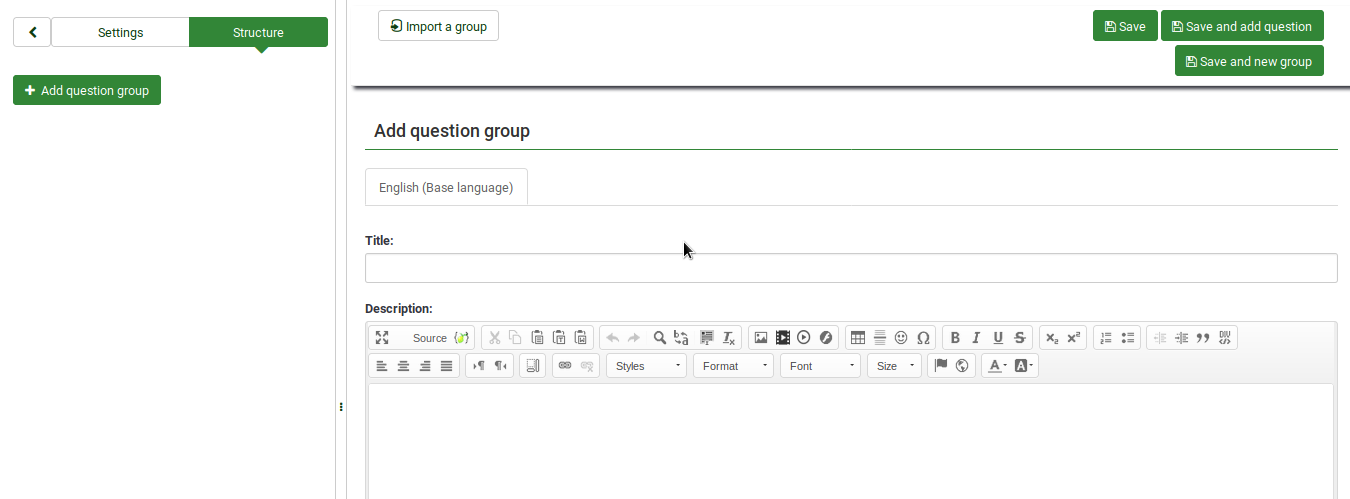
\includegraphics[scale=.35]{pics/addGroupStructure.png}
    \caption{Dialog untuk menambah kelompok pertanyaan penilaian diri}
    \label{fig:addGroupStructure}
  \end{center}
\end{figure}

Untuk menambahkan pertanyaan, beberapa informasi yang harus diberikan adalah sebagai berikut.
\begin{enumerate}
  \item Pertanyaan serta kodenya (\figurename~\ref{fig:pertanyaanDanKode}).\\
  \begin{figure}
    \begin{center}
      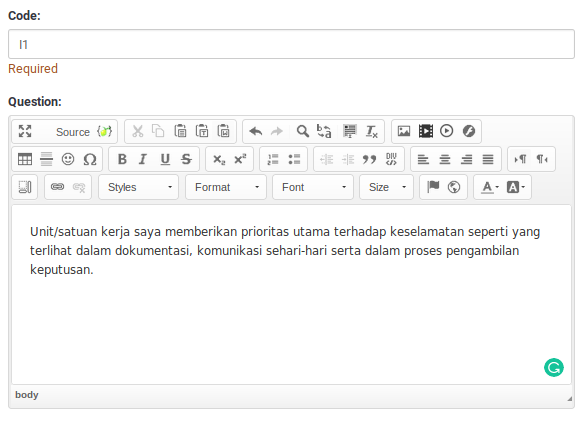
\includegraphics[scale=.5]{pics/pertanyaanDanKode.png}
      \caption{Pertanyaan dan kode dari pertanyaan tersebut}
      \label{fig:pertanyaanDanKode}
    \end{center}
  \end{figure}
  \item Memilih jenis jawaban (melalui dialog seperti \figurename~\ref{fig:jenisRespon}) serta wajib tidaknya sebuah pertanyaan dijawab. Keduanya dapat dikonfigurasi melalui menu seperti terlihat pada \figurename~\ref{fig:jenisPertanyaan}. Terkait budaya keselamatan, semua pertanyaan bersifat wajib untuk diisi (\texttt{Mandatory}).\\
  \begin{figure}
    \begin{center}
      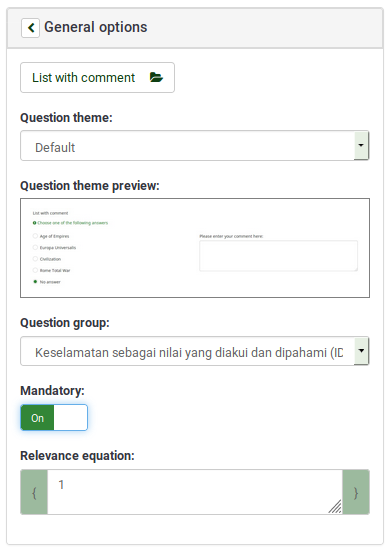
\includegraphics[scale=.5]{pics/jenisPertanyaan.png}
      \caption{Menu konfigurasi jenis jawaban}
      \label{fig:jenisPertanyaan}
    \end{center}
  \end{figure}
  \item Menambahkan petunjuk agar responden memberikan sebagai pelengkap dari pilihan responnya (\figurename~\ref{fig:komentar}). Diharapkan, responden akan berhadapan dengan pilihan jawaban dan kolom komentar seperti diilustrasikan \figurename~\ref{fig:jenisRespon}.\\
  \begin{figure}
    \begin{center}
      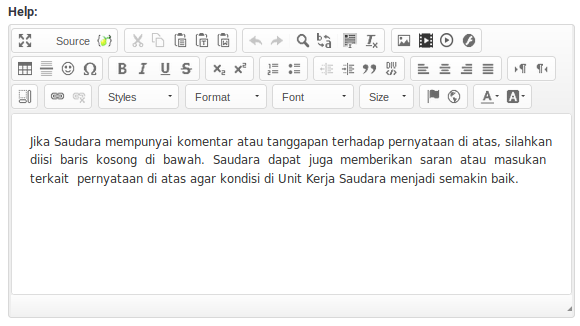
\includegraphics[scale=.5]{pics/komentarResponden.png}
      \caption{Petunjuk untuk memberikan komentar}
      \label{fig:komentar}
    \end{center}
  \end{figure}
  \begin{figure}
    \begin{center}
      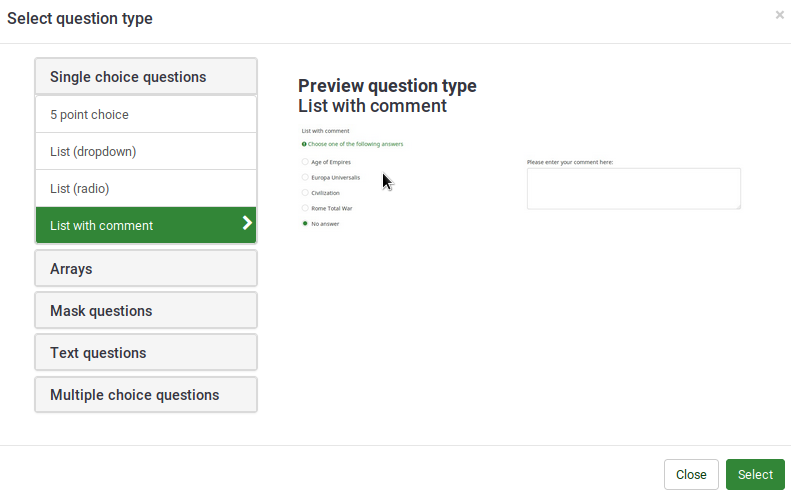
\includegraphics[scale=.5]{pics/jenisRespon.png}
      \caption{Jenis jawaban yang digunakan dalam penilaian diri budaya keselamatan}
      \label{fig:jenisRespon}
    \end{center}
  \end{figure}
  \item Jika sudah yakin, pertanyaan dapat disimpan. Sedangkan jika terdapat kesalahan, pertanyaan dapat dibatalkan. Menyimpannya (\texttt{Save}) atau membatalkan (\texttt{Close}) dilakukan melalui menu di sisi kanan atas seperti diilustrasikan \figurename~\ref{fig:savePertanyaan}.\\
  \begin{figure}
    \begin{center}
      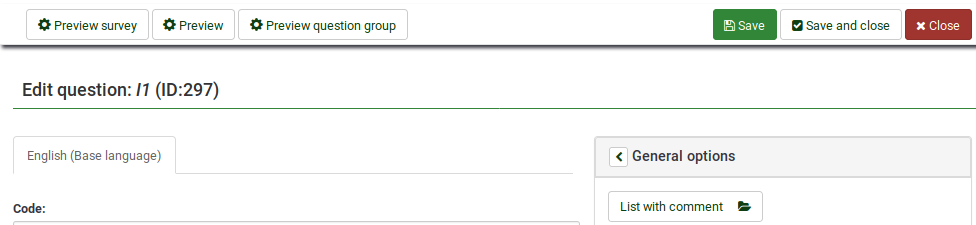
\includegraphics[scale=.5]{pics/savePertanyaan.png}
      \caption{Menu untuk menyimpan pertanyaan yang dibuat}
      \label{fig:savePertanyaan}
    \end{center}
  \end{figure}
  \item Setelah disimpan, pengelola akan menjumpai dialog seperti \figurename~\ref{fig:summaryPertanyaan}.\\
  \begin{figure}
    \begin{center}
      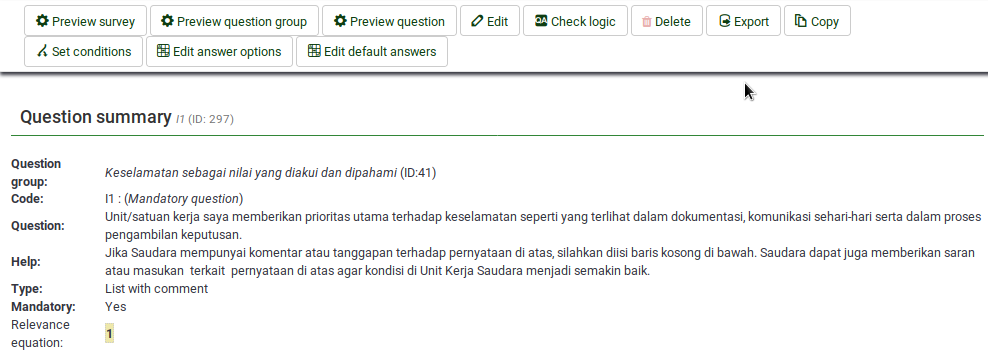
\includegraphics[scale=.5]{pics/pertanyaanSummary.png}
      \caption{Dialog berisi ringkasan pertanyaan}
      \label{fig:summaryPertanyaan}
    \end{center}
  \end{figure}
  \item Langkah terakhir adalah mengkonfigurasi opsi pertanyaan. Opsi pertanyaan ini akan digunakan untuk semua pertanyaan dalam penilaian diri. Untuk mengkonfigurasi, klik di tombol \texttt{Edit answer options} (\figurename~\ref{fig:summaryPertanyaan}). Dari tombol tersebut, pengelola akan menjumpai dialog seperti \figurename~\ref{fig:opsiPertanyaan}.\\
  \begin{figure}
    \begin{center}
      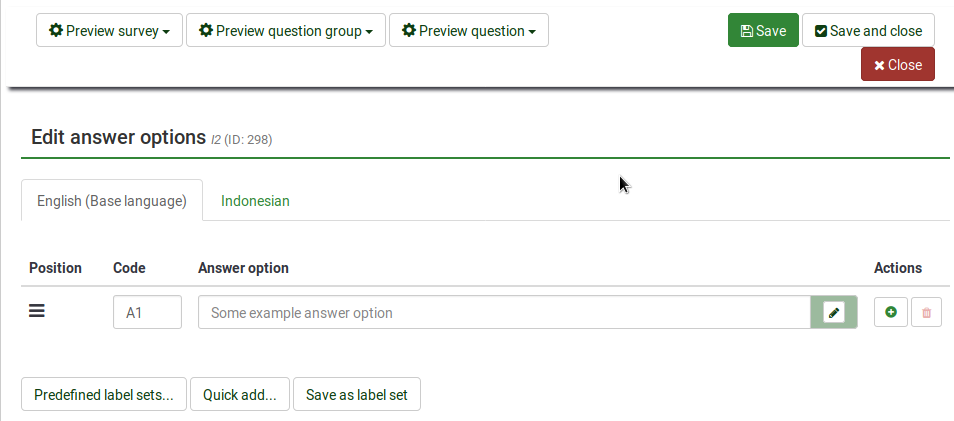
\includegraphics[scale=.5]{pics/labelSet.png}
      \caption{Menu untuk mengkonfigurasi opsi pertanyaan}
      \label{fig:opsiPertanyaan}
    \end{center}
  \end{figure}
  Dari dialog tersebut, klik pada tombol \texttt{Predefined label sets...} untuk memunculkan menu seperti \figurename~\ref{fig:labelBudkes}. Pilih label \texttt{budkesLabel}, kemudian klik tombol \texttt{Replace}. Dengan melakukan klik tombol \texttt{Replace}, menu seperti \figurename~\ref{fig:opsiPertanyaan} akan berubah menjadi \figurename~\ref{fig:labelBudkes1}. Anda dapat menyimpan pertanyaan dengan melakukan klik pada tombol \texttt{Save} di sisi kanan atas.
  
  \begin{figure}
    \begin{center}
      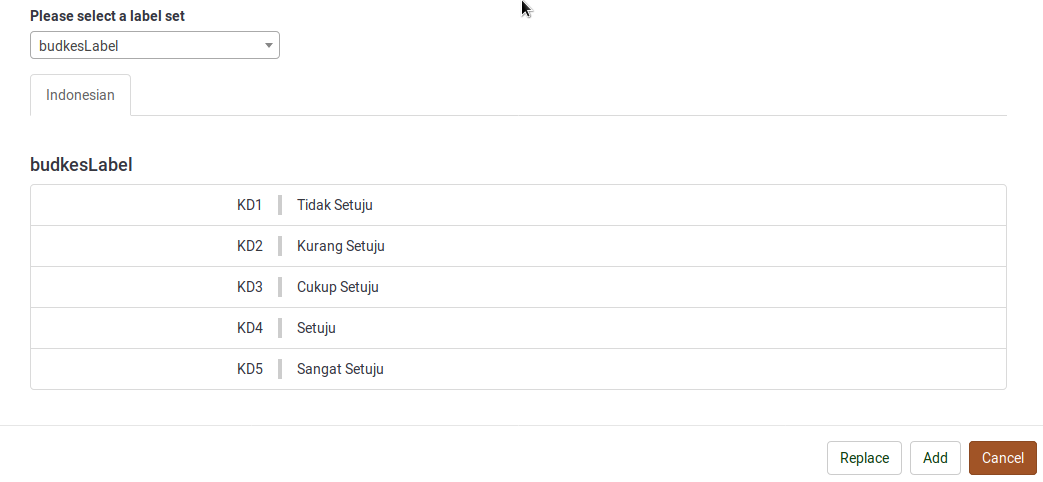
\includegraphics[scale=.5]{pics/labelSet1.png}
      \caption{Label sebagai opsi jawaban untuk penilaian diri Budaya Keselamatan}
      \label{fig:labelBudkes}
    \end{center}
  \end{figure}
  
  \begin{figure}
    \begin{center}
      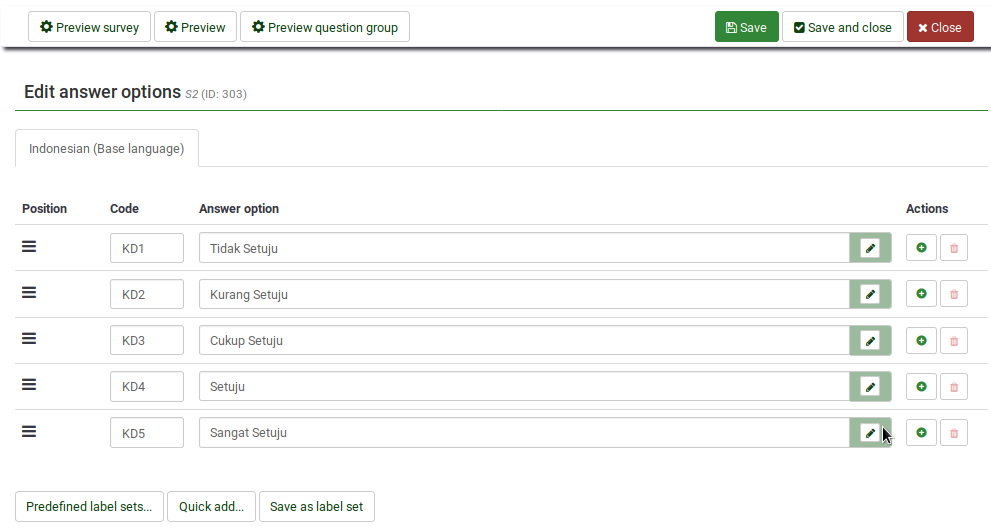
\includegraphics[scale=.5]{pics/labelSet2.png}
      \caption{Pertanyaan penilaian diri telah mendapatkan opsi jawaban}
      \label{fig:labelBudkes1}
    \end{center}
  \end{figure}
\end{enumerate}

\section{Membuat penilaian diri dari \textit{template}}
Cara pertama adalah dengan mengunggah struktur penilaian diri hasil \textit{export} dari penilaian diri yang pernah dibuat. Dialog untuk melakukannya berada pada menu tab \texttt{Import} seperti \figurename~\ref{fig:import}. Pengelola dapat memilih berkas penilaian diri kemudian melakukan klik pada tombol \texttt{Import survey}.

\begin{figure}
  \begin{center}
    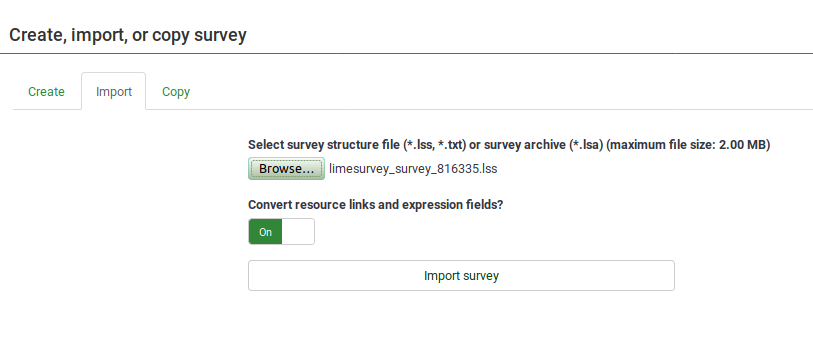
\includegraphics[scale=.5]{pics/importSurvey.png}
    \caption{\textit{Import} penilaian diri}
    \label{fig:import}
  \end{center}
\end{figure}

Proses \textit{import} tersebut hanya dapat dilakukan jika struktur pertanyaan dari penilaian diri terdahulu pernah diekspor (diunduh) dalam bentuk berkas. Untuk melakukannya, dari menu konfigurasi umum sebuah proyek penilaian diri, klik pada tombol \texttt{Display/export} seperti \figurename~\ref{fig:exportSurvey}. 

\begin{figure}
  \begin{center}
    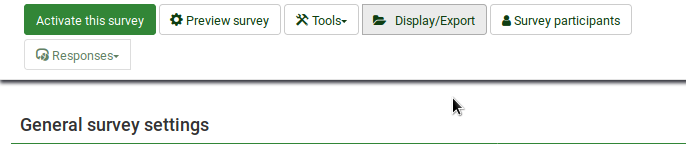
\includegraphics[scale=.5]{pics/exportSurvey.png}
    \caption{Ekspor proyek penilaian diri}
    \label{fig:exportSurvey}
  \end{center}
\end{figure}

Setelahnya, akan muncul dialog seperti pada \figurename~\ref{fig:exportSurvey1}. Silakan memilih menu Survey \texttt{structure (.lss)} lalu kemudian klik pada tombol \texttt{Export}.

\begin{figure}
  \begin{center}
    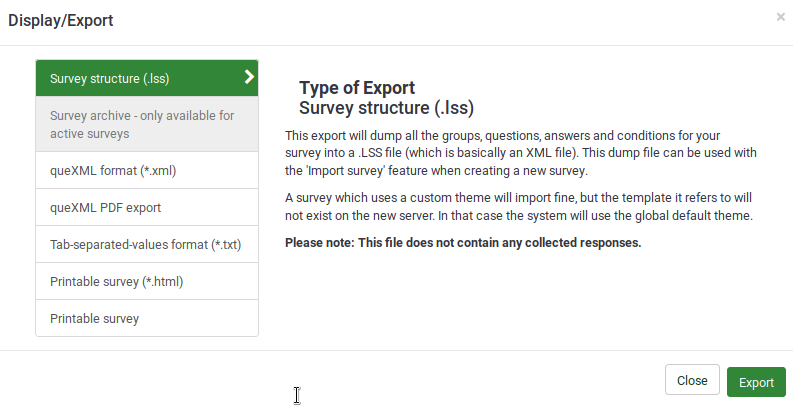
\includegraphics[scale=.5]{pics/exportSurvey1.png}
    \caption{Menu untuk ekspor penilaian diri}
    \label{fig:exportSurvey1}
  \end{center}
\end{figure}

Selain itu, penilaian diri dapat juga dibuat dengan menduplikasi penilaian diri yang pernah dibuat. Caranya seperti ditunjukkan \figurename~\ref{fig:copy}. Pilih terlebih dahulu penilaian diri yang akan diduplikasi. Setelah itu, klik pada tombol \texttt{Copy survey}.

\begin{figure}
  \begin{center}
    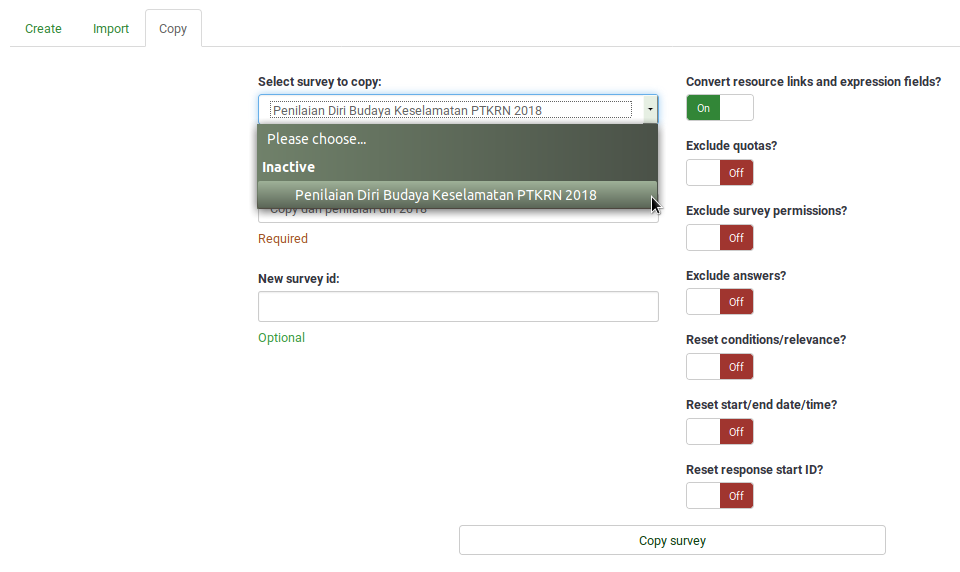
\includegraphics[scale=.35]{pics/copySurvey.png}
    \caption{Menduplikasi penilaian diri}
    \label{fig:copy}
  \end{center}
\end{figure}

Karena sifatnya yang menduplikasi penilaian diri terdahulu, maka ada beberapa parameter yang perlu dimodifikasi, salah satunya adalah judul dari penilaian diri. Hal ini bisa diganti melalui menu \texttt{Text elements} seperti ditunjukkan \figurename~\ref{fig:gantiJudul}.

\begin{figure}
  \begin{center}
    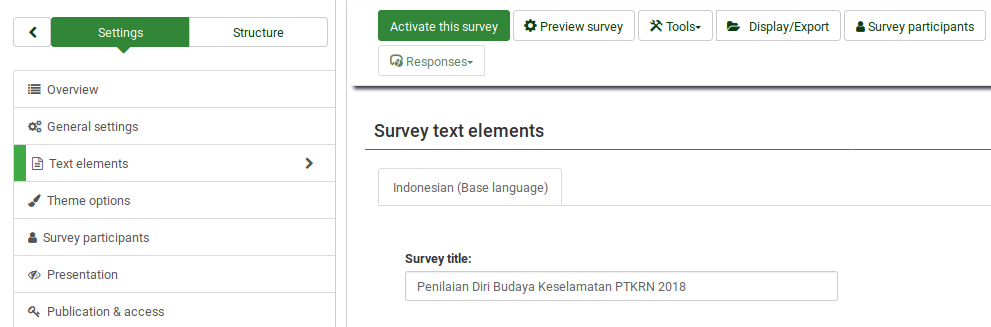
\includegraphics[scale=.5]{pics/modifSurveyTitle.png}
    \caption{Mengubah judul penilaian diri}
    \label{fig:gantiJudul}
  \end{center}
\end{figure}

\section{Mengelola responden}
Langkah selanjutnya adalah mengelola responden. Yang pertama harus dilakukan adalah mengaktifkan tabel daftar responden dengan cara klik pada tab \texttt{Survey participants}. Pada \figurename~\ref{fig:modifSurvey}, tab tersebut diberi lingkaran merah. Pengelola selanjutnya akan menemui dialog konfirmasi seperti \figurename~\ref{fig:tabelResponden}. Jika setuju, klik pada tombol \texttt{Initialize participant table}. 

\begin{figure}
  \begin{center}
    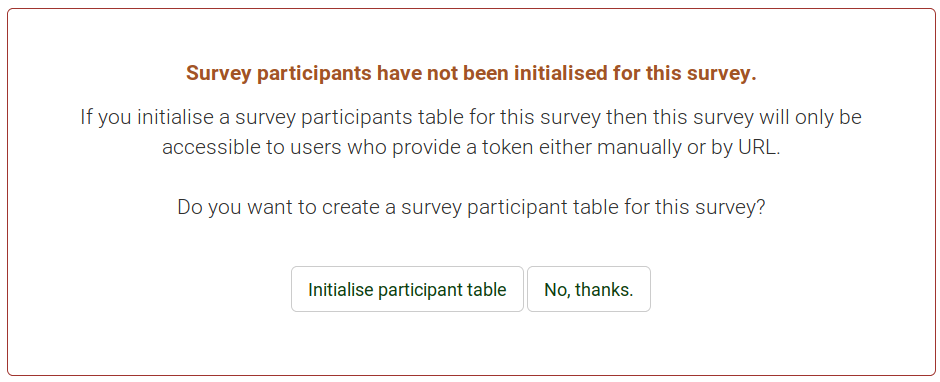
\includegraphics[scale=.35]{pics/konfirmasiPartisipan.png}
    \caption{Dialog konfirmasi pembuatan tabel responden}
    \label{fig:tabelResponden}
  \end{center}
\end{figure}

Pengelolapun selanjutnya akan menemui dialog seperti \figurename~\ref{fig:tabelResponden1}. Angka 888564 dalam dialog tersebut merupaka identitas penilaian diri yang diberikan oleh aplikasi. Berikan klik pada tombol \texttt{Continue}.

\begin{figure}
  \begin{center}
    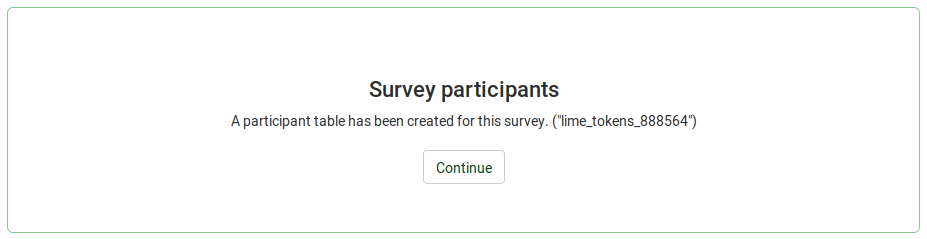
\includegraphics[scale=.5]{pics/konfirmasiPartisipan1.png}
    \caption{Dialog konfirmasi tabel responden telah dibuat oleh aplikasi}
    \label{fig:tabelResponden1}
  \end{center}
\end{figure}

Kemudian, aplikasi akan menampilkan dialog seperti \figurename~\ref{fig:addResponden}, di mana pengelola dapat menambahkan responden, baik satu per satu (menu dengan garis merah) maupun sekaligus (menu dengan warna latar hijau).

\begin{figure}
  \begin{center}
    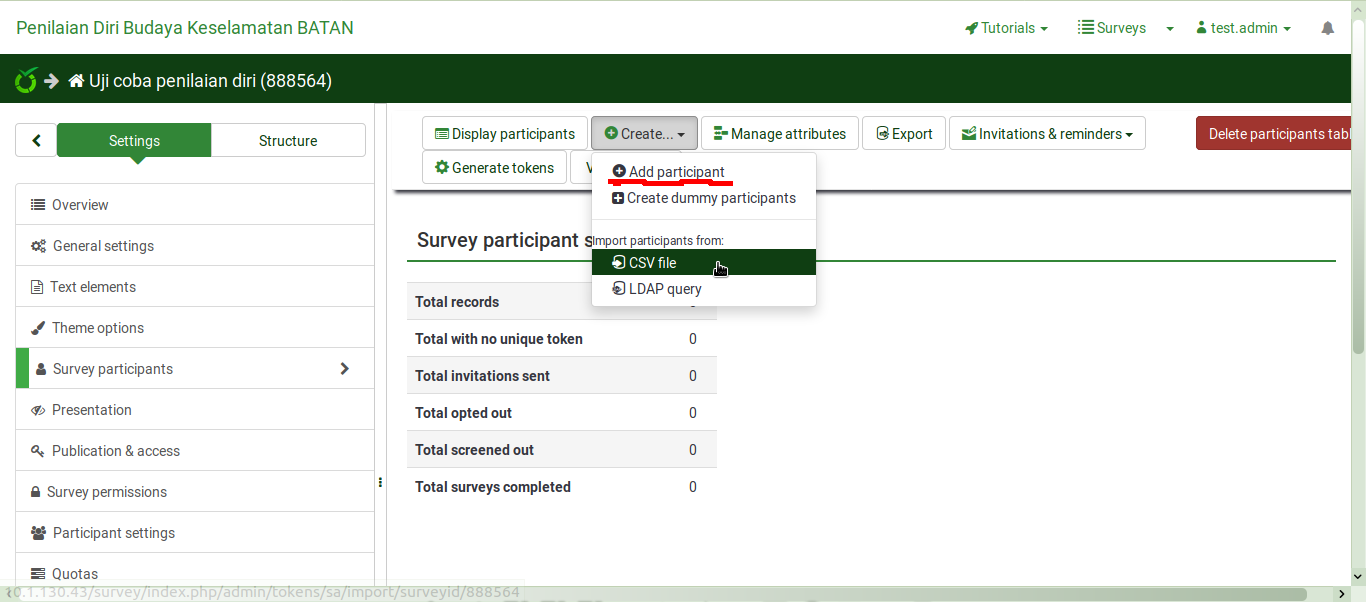
\includegraphics[scale=.25]{pics/addResponden.png}
    \caption{Dialog untuk menambahkan responden dalam penilaian diri}
    \label{fig:addResponden}
  \end{center}
\end{figure}

Jike menu \texttt{Add participant} yang dipilih, pengelola akan menjumpai dialog seperti \figurename~\ref{fig:addResponden1}. Informasi utama yang harus diberikan adalah alamat surat elektronik serta rentang waktu valid. Setelah informasi tersebut diberikan, simpan dengan melakukan klik pada tombol \texttt{Save}.

\begin{figure}
  \begin{center}
    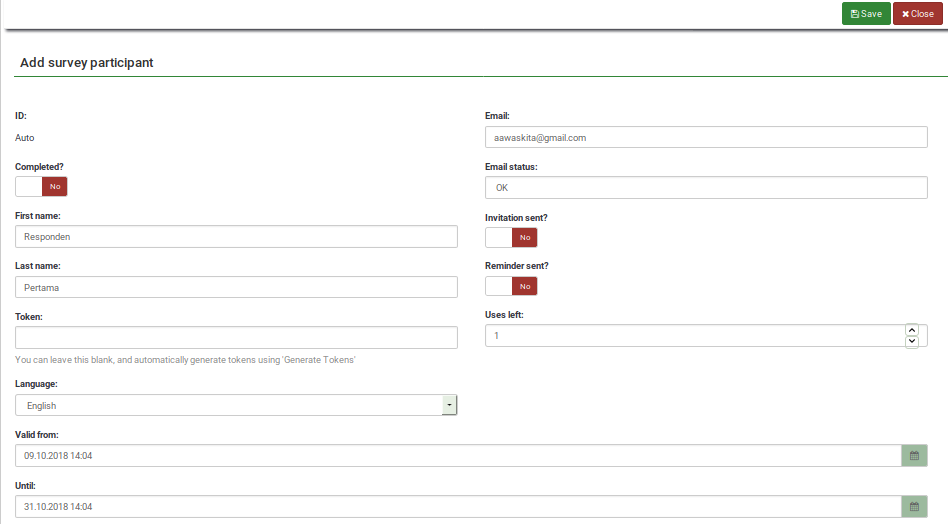
\includegraphics[scale=.5]{pics/addResponden1.png}
    \caption{Menambahkan responden satu persatu}
    \label{fig:addResponden1}
  \end{center}
\end{figure}

Sedangkan jika pengelola akan memasukkan beberapa responden sekaligus, gunakan menu \texttt{CSV file} yang memiliki warna latar hijau pada \figurename~\ref{fig:addResponden1}. Dialog seperti \figurename~\ref{fig:csv} akan muncul kemudian. 

\begin{figure}
  \begin{center}
    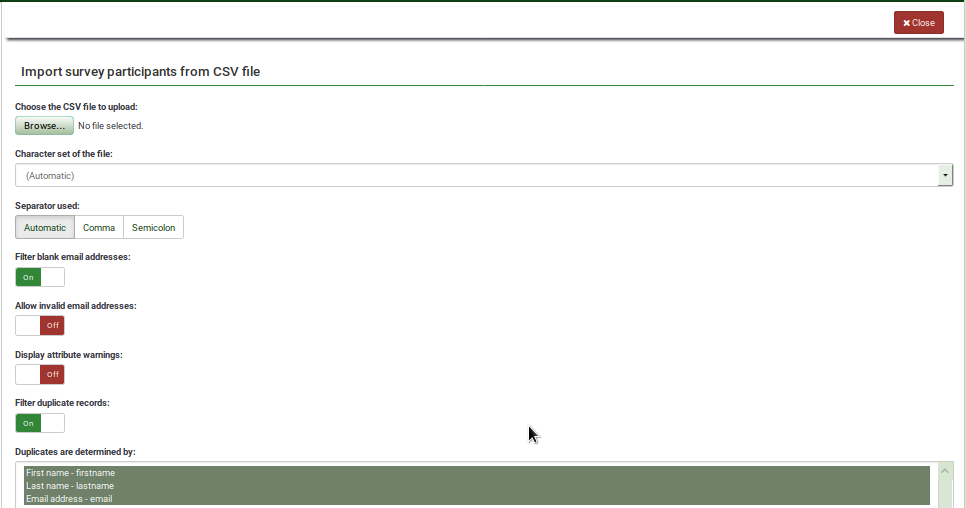
\includegraphics[scale=.5]{pics/csvFile.png}
    \caption{Dialog untuk menambahkan sejumlah responden sekaligus melalui berkas csv}
    \label{fig:csv}
  \end{center}
\end{figure}

Yang perlu diperhatikan adalah berkas csv yang dibuat harus diawali dengan keterangan kolom yang masing-masing adalah \texttt{firstname}, \texttt{lastname} dan \texttt{email}. \figurename~\ref{fig:csvFile1} mengilustrasikan berkas csv berisi nama dan alamat surat elektronik responden untuk ditambahkan ke aplikasi. 

\begin{figure}
  \begin{center}
    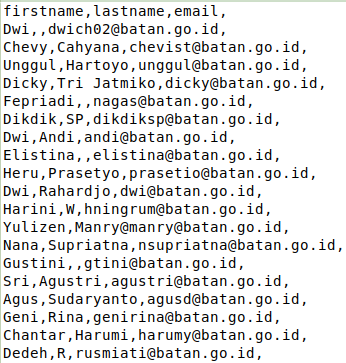
\includegraphics[scale=.5]{pics/csvFile1.png}
    \caption{Format berkas csv berisi nama dan surat elektronik responden}
    \label{fig:csvFile1}
  \end{center}
\end{figure}

Berkas csv tersebut kemudian diunggah ke aplikasi. Pastikan bahwa pengelola telah memilih berkas yang tepat untuk kemudian melakukan klik pada tombol \texttt{Upload} (\figurename~\ref{fig:csvFile2}). Hasilnya disajikan pada \figurename~\ref{fig:addResponden2}.

\begin{figure}
  \begin{center}
    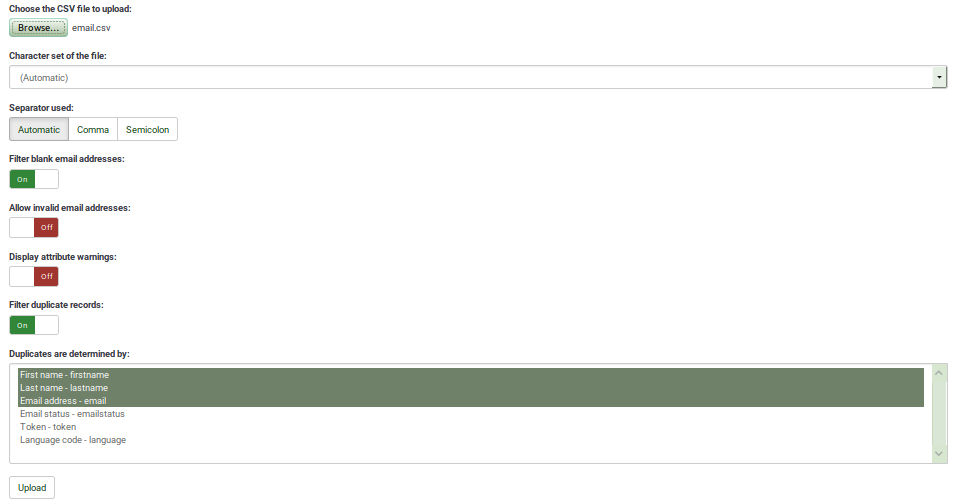
\includegraphics[scale=.5]{pics/csvFile2.png}
    \caption{Pastikan memilih berkas yang tepat lalu klik pada tombol \texttt{Upload}}
    \label{fig:csvFile2}
  \end{center}
\end{figure}

\begin{figure}
  \begin{center}
    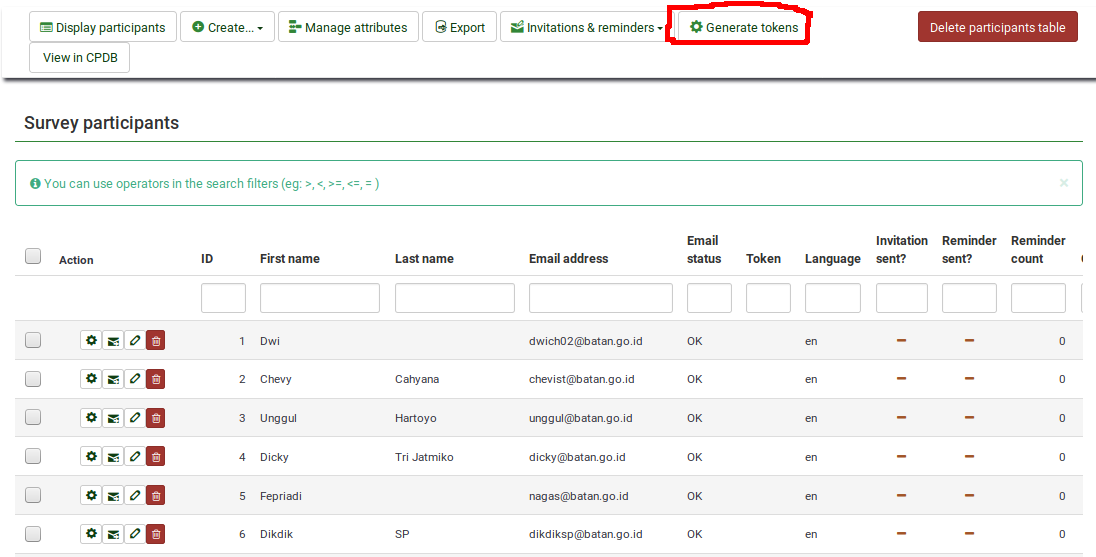
\includegraphics[scale=.5]{pics/addResponden2.png}
    \caption{Daftar responden yang telah ditambahkan ke aplikasi penilaian diri}
    \label{fig:addResponden2}
  \end{center}
\end{figure}

Untuk melengkapi tahapan penambahan responden, pengelola harus membangkitkan serangkaian karakter acak yang berperan sebagai identitas responden. Karakter acak tersebut adalah \textit{token}. Membangkitkan \textit{token} untuk responden dilakukan dengan memberikan klik pada tombol \texttt{Generate tokens} (dalam lingkaran merah) pada \figurename~\ref{fig:addResponden2}. Dari situ, muncul dialog konfirmasi untuk membangkitkan \textit{token} seperti \figurename~\ref{fig:generateTokens}.

\begin{figure}
  \begin{center}
    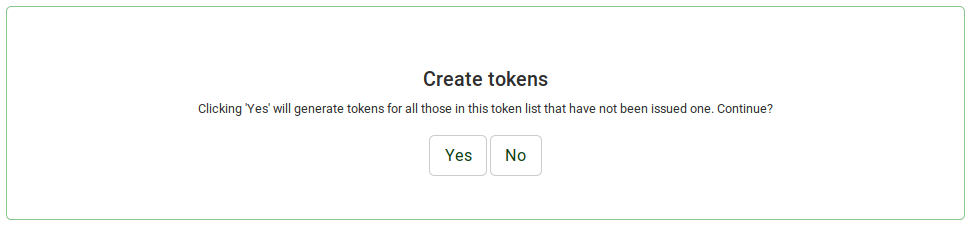
\includegraphics[scale=.5]{pics/konfirmasiTokens.png}
    \caption{Konfirmasi pembangkitan \textit{tokens}}
    \label{fig:generateTokens}
  \end{center}
\end{figure}

Jika yakin akan membangkitkan \textit{token}, klik tombol \texttt{Yes} pada \figurename~\ref{fig:generateTokens}. Selanjutnya, dialog konfirmasi bahwa \textit{token} telah dibangkitkan akan muncul seperti \figurename~\ref{fig:tokenGenerated}.

\begin{figure}
  \begin{center}
    
\includegraphics[scale=.5]{pics/tokenGenerated.png}
    \caption{Konfirmasi \textit{token} telah berhasil dibangkitkan}
    \label{fig:tokenGenerated}
  \end{center}
\end{figure}

Terakhir, penilaian diri harus diaktifkan melalui menu seperti \figurename~\ref{fig:aktivasi}. 

\begin{figure}
  \begin{center}
    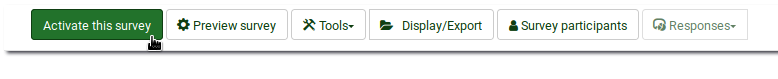
\includegraphics[scale=.5]{pics/aktivasiSurvey.png}
    \caption{Aktivasi penilaian diri}
    \label{fig:aktivasi}
  \end{center}
\end{figure}

Kemudian, akan muncul dialog konfirmasi seperti \figurename~\ref{fig:konfirmasiAktivasi}. Pastikan untuk memilih opsi \texttt{No} untuk \texttt{Anonymized responses?}. 

\begin{figure}
  \begin{center}
    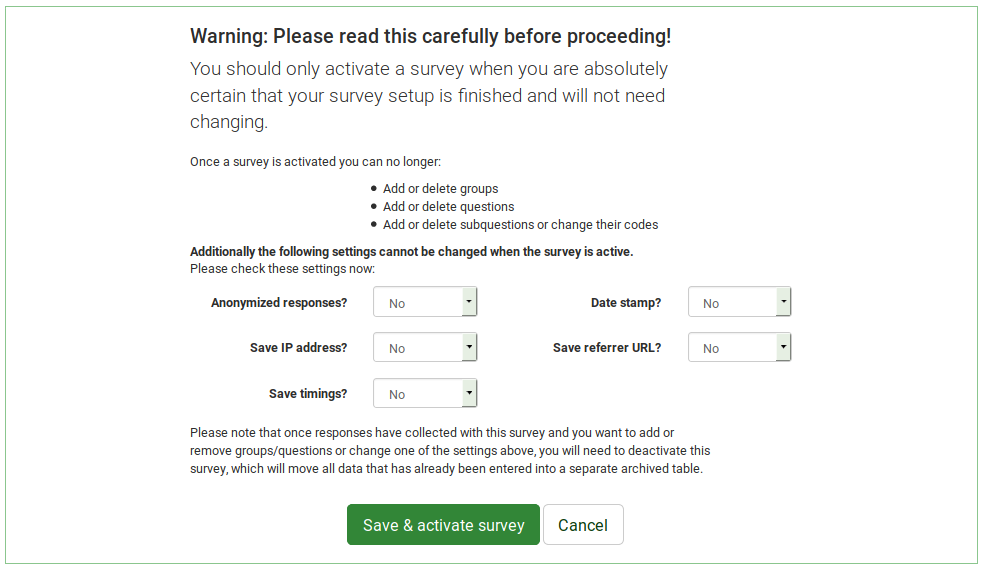
\includegraphics[scale=.35]{pics/konfirmasiAktivasi.png}
    \caption{Konfirmasi aktivasi penilaian diri}
    \label{fig:konfirmasiAktivasi}
  \end{center}
\end{figure}

Bila aktivasi berhasil, akan muncul konfirmasi seperti \figurename~\ref{fig:aktivasiBerhasil} berikut.

\begin{figure}
  \begin{center}
    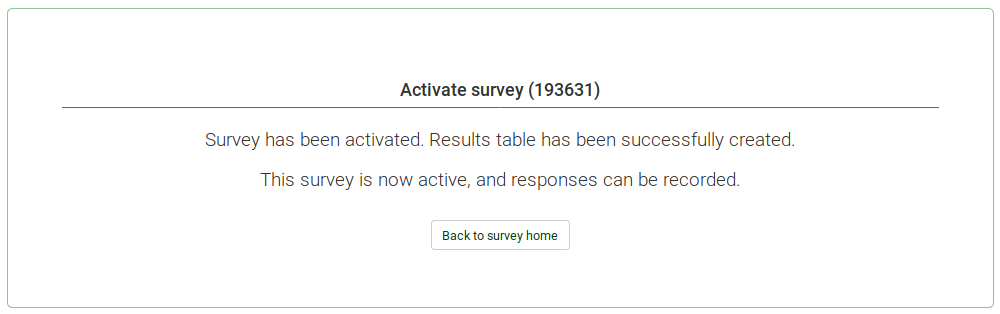
\includegraphics[scale=.5]{pics/aktivasiBerhasil.png}
    \caption{Aktivasi berhasil dilakukan}
    \label{fig:aktivasiBerhasil}
  \end{center}
\end{figure}

\section{Mengirimkan undangan}
Untuk mengirimkan undangan partisipasi dalam penilian diri, dapat dilakukan melalui menu seperti \figurename~\ref{fig:undangan}. Dari menu tersebut, dapat juga dimanfaatkan untuk mengirimkan pengingat bagi responden yang telah dikirimkan undangan tetapi belum melakukan penilaian diri. Dialog untuk mengirimkan undangan berpartisipasi akan muncul seperti \figurename~\ref{fig:undangan1}. Di \figurename~\ref{fig:undangan1} tersebut, format undangan selain dapat dibuat melalui editor yang disediakan, dapat juga dibuat melalui menu \texttt{Email templates} di sisi kiri.

\begin{figure}
   \begin{center}
     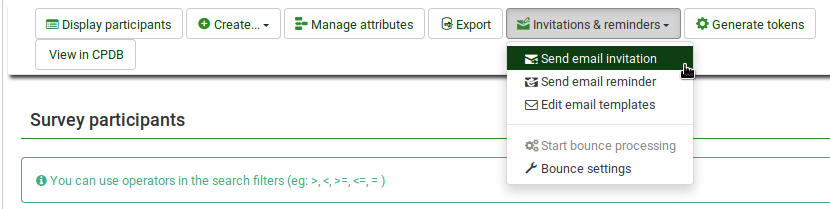
\includegraphics[scale=.5]{pics/undangan.png}
     \caption{Menu untuk mengundang responden}
     \label{fig:undangan}
   \end{center}
 \end{figure} 
 
 \begin{figure}
   \begin{center}
     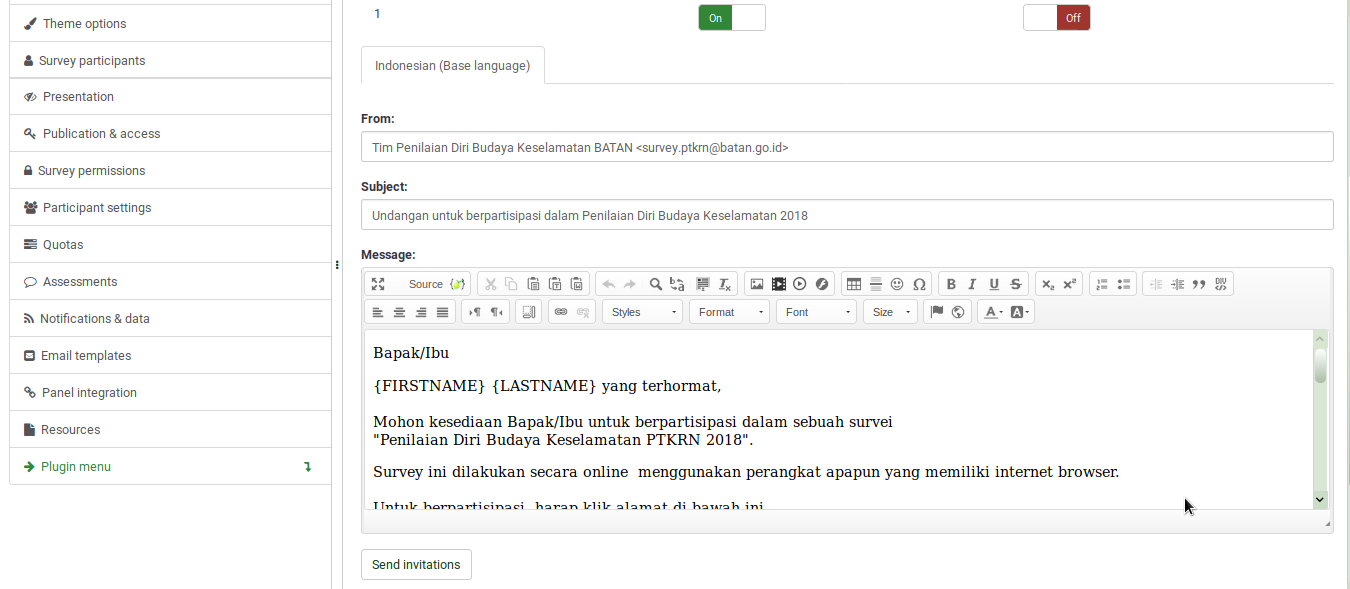
\includegraphics[scale=.35]{pics/undangan1.png}
     \caption{Konfigurasi undangan berpartisipasi}
     \label{fig:undangan1}
   \end{center}
 \end{figure}
 
 Setelah undangan dikirim, akan muncul konfirmasi seperti \figurename~\ref{fig:undangan2}. Konfirmasi tersebut dikeluarkan baik untuk kondisi berhasil terkirim maupun gagal.
 
 \begin{figure}
   \begin{center}
     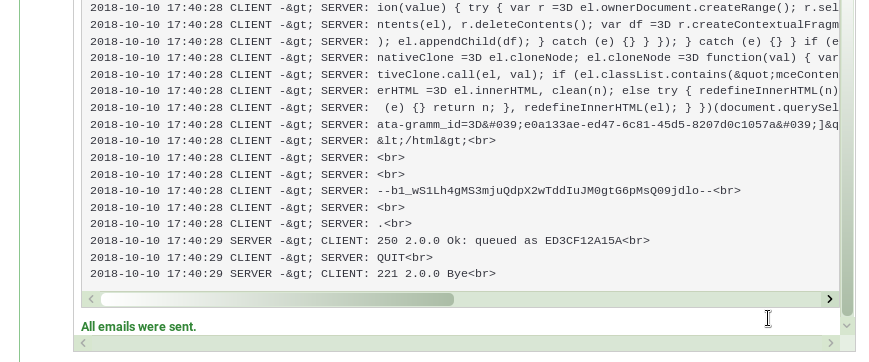
\includegraphics[scale=.5]{pics/undangan2.png}
     \caption{Konfirmasi bahwa undangan telah berhasil dikirim}
     \label{fig:undangan2}
   \end{center}
 \end{figure}
 
 Undangan terkirim melalui surat elektronik seperti \figurename~\ref{fig:undangan3}. Yang perlu diperhatikan adalah tautan alamat penilaian diri bagi responden yang ada di bagian bawah surat elektronik. Alamat tautan tersebut yang menjadi media bagi responden melakukan penilaian diri. Jika pada kondisi tertentu, terdapat responden yang jarang, kesulitan mengakses surat elektroniknya (mungkin karena lupa kata sandi) atau bahkan untuk kondisi terbutuk sekalipun (responden tidak memiliki surat elektronik), alamat tautan dapat dikirimkan melalui media lain (WA) dengan memperhatikan kode penilaian diri dan \textit{token} dari setiap responden.
 
 \begin{figure}
   \begin{center}
     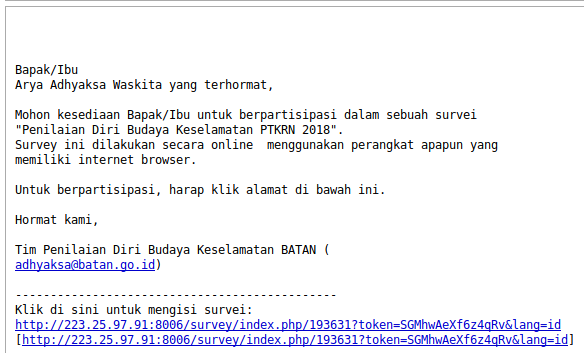
\includegraphics[scale=.5]{pics/undangan3.png}
     \caption{Undangan bagi responden}
     \label{fig:undangan3}
   \end{center}
 \end{figure}
 

 Dari contoh yang disajikan pada \figurename~\ref{fig:undangan3}, maka alamat tautan penilaian diri bagi responden tersebut adalah \url{http://223.25.97.91:8006/survey/index.php/193631?token=SGMhwAeXf6z4qRv&lang=id}. \texttt{193631} adalah ID penilaian diri, sedangkan \texttt{SGMhwAeXf6z4qRv} adalah \textit{token} bagi responden. Pengelola dapat menginformasikan kepada responden yang bermasalah dengan surat elektronik untuk ikut penilaian diri di alamat tautan \url{http://223.25.97.91:8006/survey/index.php/193631} (dengan mengganti ID penilaian diri yang sesuai) serta \textit{token} responden. Dengan mengakses alamat tautan, responden akan menjumpai halaman seperti \figurename~\ref{fig:tanpaToken}.
 
 \begin{figure}
   \begin{center}
     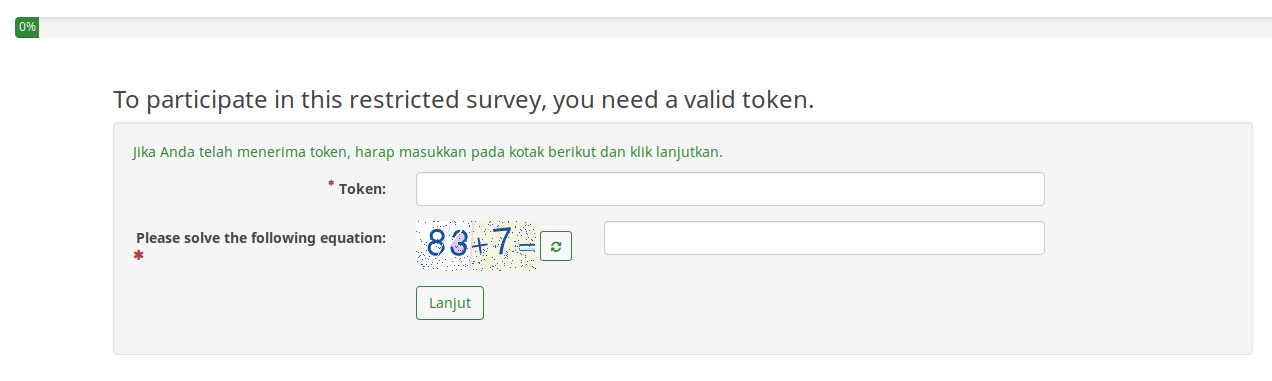
\includegraphics[scale=.4]{pics/tanpaEmail.png}
     \caption{Halaman web untuk tautan tanpa disertai \textit{token}}
     \label{fig:tanpaToken}
   \end{center}
 \end{figure}
 
